% !TEX root = ../ThesisManuscript_SJ.tex
%%
%%	VOLUNTARY VACCINATION
%%_______________________________________________
\chapter{Voluntary vaccination against treatable childhood infectious diseases} 
\label{Vaccine}
\hypertarget{Vaccine}{}
\markboth{VOLUNTARY VACCINATION}{}

\addtocontents{lof}{\protect\contentsline{chapter}{\protect\numberline{}Chapter \thechapter \medskip}{}{}}
\addtocontents{lot}{\protect\contentsline{chapter}{\protect\numberline{}Chapter \thechapter \medskip}{}{}}

\section{Introduction}
\label{Vaccine:Intro}
\subsection{Vaccines against childhood infectious diseases}
Vaccines are used to stimulate the individuals' immune system to fight infectious diseases, providing individuals with acquired immunity against the disease --- in contrast to naturally-acquired immunity, which occurs after infection and recovery. %There exists four main types of vaccines, which use attenuated, killed forms or parts of a pathogen (such as proteins, sugars, etc), or toxins produced by the pathogen (creating immunity against the disease rather than the pathogen itself). More recently, RNA messenger (mRNA) vaccines were developed to teach immune cells how to make a protein that triggers the immune response. 
%
The development of highly-effective vaccines inducing long-lasting immunity has changed the course of many epidemics~\cite[]{CDC_10achievements}. As a result, most countries have established vaccination programs, with vaccination schedules varying between countries and regions. Childhood immunization schedules (i.e., vaccines to be administered before the age of 5, or when children start attending school) currently recommended by the WHO and local public health authorities include vaccines against: measles%\footnote{The epidemiology of measles is discussed in more detail in section~\ref{sec:MeaslesEpi}, where we present an application of our model.}
, bacterial meningitis, mumps%
%\footnote{Viral infection causing the inflammation of the salivary glands. Complications may include inflammation of the heart, the pancreas and meningitis~\cite[]{CDC_PinkBook}.}
, poliomyelitis, and rubella% \footnote{Viral infection often causing mild symptoms, such as fever and a rash. However, infection during early pregnancy may result in miscarriage or severe congenital sequelae~\cite[]{CDC_PinkBook}.}
~\cite[]{CDC_PinkBook,CalendrierVaccinal2019}. 

Some of these infectious diseases have reached --- or been close to reach --- elimination status, at least regionally, thanks to high levels of vaccine coverage; see table~\ref{table:ChildInfDis}. For instance, vaccination made the eradication of smallpox possible in 1980~\cite[]{WHO_SmallpoxEradication1980,CDC_Smallpox2001}. Immunization programs reduced the number of polio cases by 99\% since 1988, worldwide. Polio was declared eliminated from the Americas in 1994, from the Western Pacific region in 2000 and from the European region in 2002. As for 2019, polio remained endemic in only 3 countries~\cite[]{WHO_Factsheet_Polio}. The combined measles-mumps-rubella (MMR) vaccine was first licensed for use in the US in 1971 and was recommended worldwide once safety and high effectiveness of the three-vaccine combination were demonstrated in different settings~\cite[]{Strebel2013}. The remarkable reduction of diseases cases inspired the worldwide priority goal to eliminate rubella and measles by 2020~\cite[]{Andrus2011,WHO_MRPlan2012}, which remains to be achieved.

As discussed in the previous chapter, epidemic control requires safe, highly-effective vaccines, as well as high levels of vaccine coverage. However, despite the large evidence of vaccine-induced reduction in the number of infections and the public health authorities' recommendations about vaccination, parents still hesitate to vaccinate their children~\cite[]{Larson2016}. Therefore, the coverage of vaccines against childhood infectious diseases remains suboptimal in many settings (that is, below the elimination threshold, the threshold to obtain herd immunity; cf. table~\ref{table:ChildInfDis}) and disease outbreaks still occur.

\begin{landscape}
\captionsetup{width=1.3\textwidth}
\begin{table}[H]
	\centering
	\small
%	\footnotesize
	\begin{tabular}{lccccc}
%	\begin{tabular}{llllll}
	\toprule
	\bf Infectious & \bf $R_0$ & \bf Year of& \bf Vaccine & \bf Herd immunity & \bf Vaccine \vspace{-4pt}\\ 
	\bf disease & & \bf licence & \bf effectiveness & \bf threshold & \bf coverage (year)\\
	\toprule
	\bf Diphtheria & 4--5 & 1930s & \phantom{$\sim$}95\%\textsuperscript{a}& 80\%--85\% & 85\%\textsuperscript{d} (2019)\\
	& \cite[]{Anderson1991} & \cite[]{CDC_PinkBook} & \cite[]{CDC_PinkBook} & \cite[]{Anderson1990} & \cite[]{WHO_Factsheet_VaccineCoverageWorldwide}\\ \midrule
%	
	\bf Measles 	& 8--18 	& 1963 & >95\%\textsuperscript{b} & 92\%--95\% & 64\% \;(2016)\\
	& \cite[]{Anderson1991} 	& \cite[]{CDC_PinkBook} & \cite[]{Plotkin2012} & \cite[]{Anderson1990} & \cite[]{WHO_HealthStats2018}\\ \midrule
%
%	\bf Mumps 	& 7--14~\cite[]{Anderson1991}  	& 1967~\cite[]{Plotkin2012} &  $\sim$ 88\%\textsuperscript{a}~\cite[]{Plotkin2012} & 85\%--90\%~\cite[]{Plotkin2012} \\
	\bf Polio 		& 5--7 & 1955 & \phantom{$\sim$}99\%\textsuperscript{c}  & 80\%--85\% & 86\%\textsuperscript{c } (2019)\\
	& \cite[]{Anderson1991}  	& \cite[]{Plotkin2012} & \cite[]{CDC_PinkBook}  & \cite[]{Anderson1990} & \cite[]{WHO_Factsheet_VaccineCoverageWorldwide} \\ \midrule
%
	\bf Rubella 	& 6--16	& 1969 &  $\sim$100\%  & 85\%--87\% & 71\% \;(2019)\\
	& 6\cite[]{Anderson1991}  	& \cite[]{CDC_PinkBook} & \cite[]{Plotkin2012}  & \cite[]{Anderson1990} & \cite[]{WHO_Factsheet_VaccineCoverageWorldwide}\\ \midrule
%
%	\bf Meningitis\textsuperscript{b} & & \% &  \% & <50\% (2016) &\cite[]{WHO_HealthStats2018}\\
%	\bf Pertussis 	& &  \% & 86\% &\cite[]{WHO_HealthStats2018}\\
%
	\bf Smallpox & 3--10 & 1796 & \phantom{$\sim$}95\% & 66\%--70\% & \multicolumn{1}{c}{$\ast$}\\
	& \cite[]{Plotkin2012} & \cite[]{WHO_SmallpoxVaccines} & \cite[]{CDC_Factsheet_Smallpox} & \cite[]{Plotkin2012} & \\
	\bottomrule
\end{tabular}
	\caption[Key data on vaccination against some preventable childhood infectious diseases, worldwide]{%
	\textbf{Key data on vaccination against some preventable childhood infectious diseases, worldwide.}\\ Basic reproduction number ($R_0$), year of vaccine development (or year of first use as preventive method), vaccine effectiveness, vaccine coverage required to reach herd immunity and vaccine coverage reached worldwide.\\
	\textsuperscript{a}After four spaced doses between 2 and 18 months old.\\
	\textsuperscript{b}After two shortly separated doses.\\
	\textsuperscript{c}After three doses of inactivated poliovirus vaccine.\\
	\textsuperscript{d}Corresponding to three doses.\\
	$^\ast$Eradication declared in 1980~\cite[]{WHO_SmallpoxEradication1980}. Smallpox eradication was reached through massive inoculation programs, initially aiming to reach at least 80\% in 1966, then aiming to reach a 100\% coverage~\cite[]{Plotkin2012}.
	}
	\label{table:ChildInfDis}
\end{table}
\end{landscape}

\subsection{Vaccine hesitancy}

Vaccine hesitancy is defined by the WHO as the ``delay in acceptance or refusal of vaccines despite availability of vaccine services''~\cite[]{WHO_VaccineHesitancy2014}. In 2019, the WHO listed vaccine hesitancy among the ten threats to global health~\cite[]{WHO_10challenges2019}. The underlying causes for vaccine hesitancy vary widely, from misinformation, to undesired effects, safety concerns, healthcare system mistrust, social pressure, religious convictions, etc.~\cite[]{Brown2010,Dube2013,Larson2014,Dube2018,Quinn2019}. 

A large-scale survey on confidence in immunization conducted in 2015 found that, while the state of vaccine confidence is overall high worldwide, there are regions where vaccine hesitancy remains a public health challenge~\cite[]{Larson2016}; see~\figref{fig:Vacc_FigLarson2016}. %Mistrust in immunization concerned both low- and high-income countries. 
Seven of the ten least confident countries were identified in the European region. France was identified as the country having the lowest confidence in vaccine safety, between the 67 countries included in the survey. Indeed, $45.2\%$ of French respondents reported mistrust in vaccine safety (of note, the global average was $13\%$)~\cite[]{Larson2016}.

\begin{figure}[H]
	\centering	
	%% DRAFT
%	
\includegraphics[width=0.6\textwidth]{DRAFT_FigsAndDocs/FIG}
	%%
	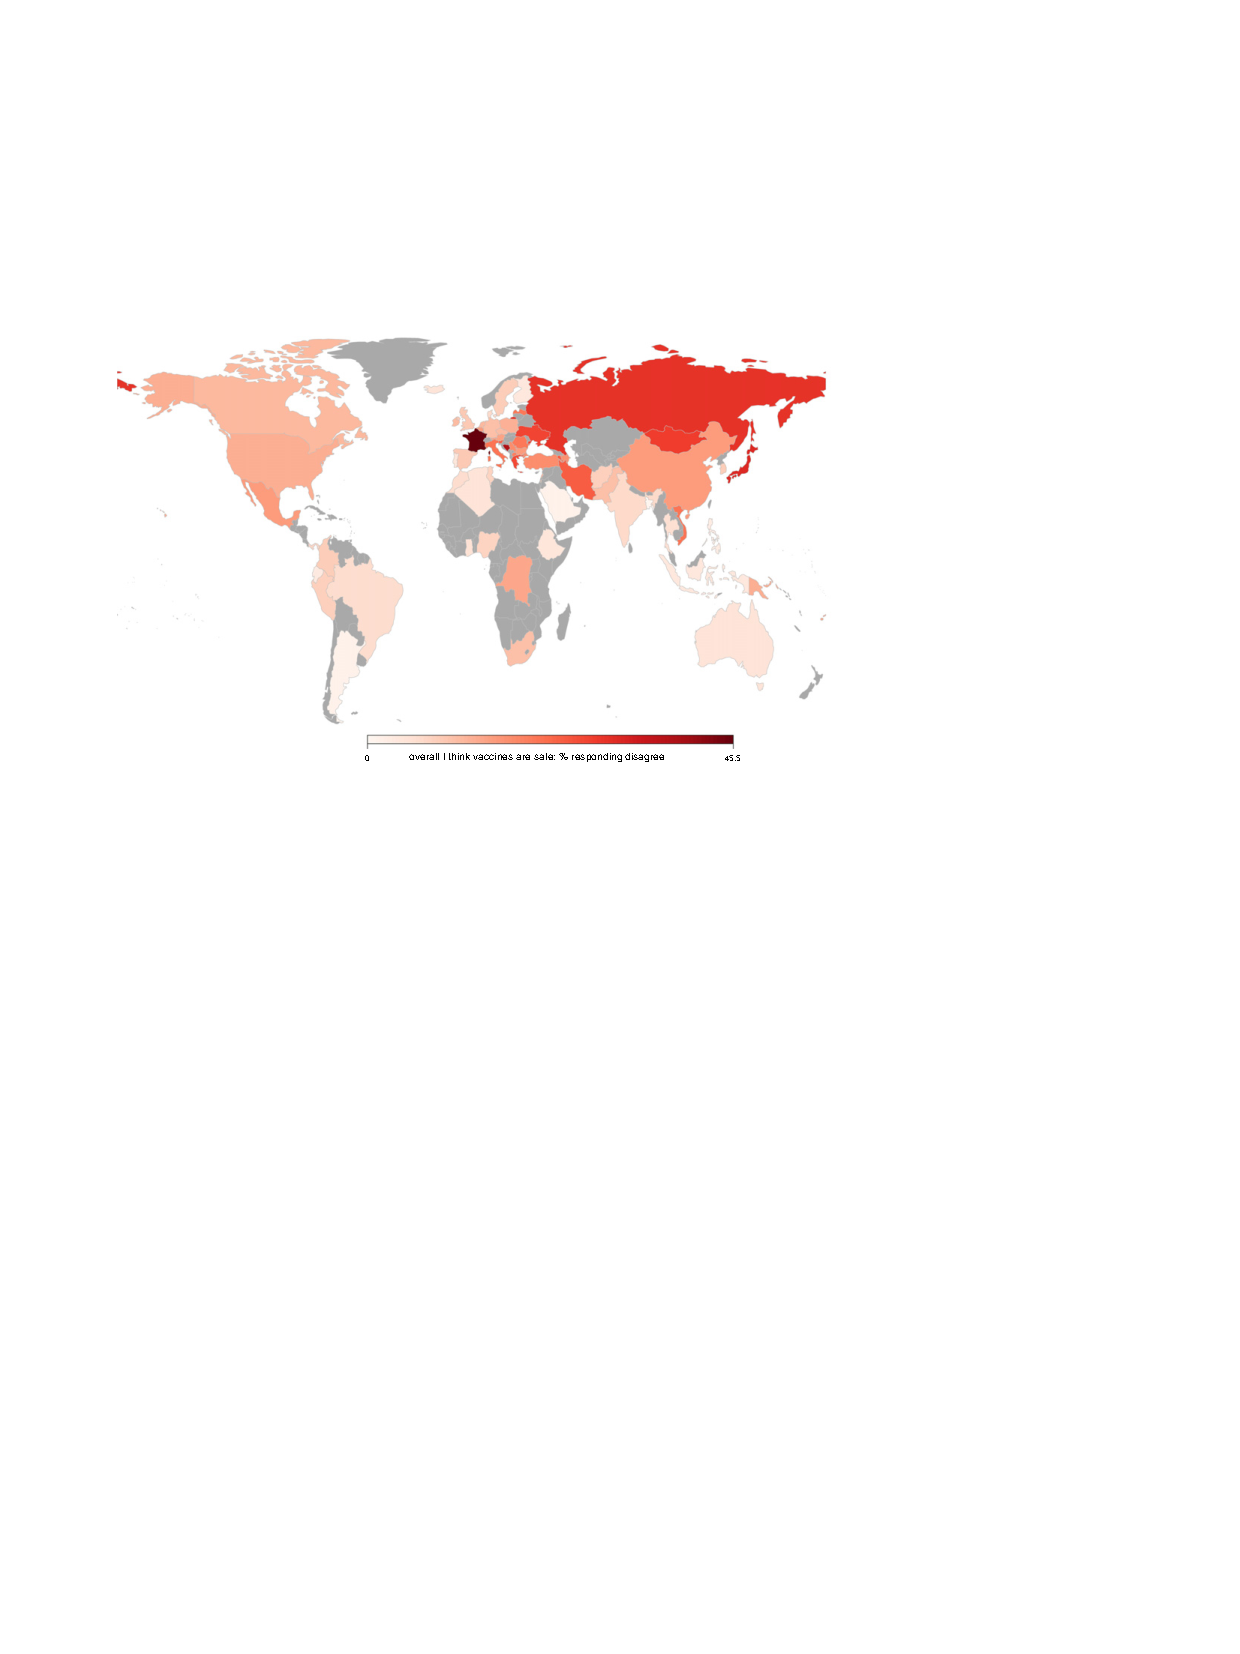
\includegraphics[width=0.8\textwidth, trim={0 0 0 4mm}, clip=true]{Figures/Vaccine/Fig_Larson2016}
	\caption[ Immunization confidence, worlwide]{%
		{\bf Immunization confidence, worlwide}\\
		World map of the percentage of negative responses (``tend to disagree'' or ``strongly agree'') to the survey the statement ``overall I think vaccines are safe''. Figure adapted from Ref.~\cite[]{Larson2016}.}
	\label{fig:Vacc_FigLarson2016}
\end{figure}

%\rev{Finding strategies for addressing vaccine hesitancy has thus become a key global health challenge~\cite[]{WHO_VaccineHesitancy2014}.  }

%The parental attitudes towards childhood vaccination may vary widely between individuals and depend on the particularities of the different available vaccines, which poses difficulties in proposing a unique way to address vaccine hesitancy~\cite[]{Dube2013}. The interventions used include dialogue-based interventions (such as social mobilization, information through mass media, etc.), non-financial incentives and reminder activities~\cite[]{Jarrett2015,WHO_VaccineHesitancy2014}. The low trust in vaccination yielding low levels of vaccination coverage has also risen debates on whether mandatory vaccination should be imposed over voluntary vaccination~\cite[]{Dube2013,Quinn2019,Bechini2019}.

Childhood-vaccine hesitancy may result in a decline in vaccination coverage, which may reach sub-optimal levels and lead to outbreaks of infectious diseases otherwise controlled, such as measles~\cite[]{Strebel2013}. Indeed, as of 2017, twelve countries of the European Union (EU) had reported a decrease in the MMR vaccine coverage~\cite[]{Larson2018}. Parents declining MMR vaccination for their children have declared to mistrust vaccines' safety and effectiveness, as well as believing that the diseases they prevent are mild and uncommon~\cite[]{Brown2010}. Hence, measles vaccination coverage and incidence are considered as tracers of the strength of immunization programs for the 2030 SDG~\cite[]{WHO_IA2030}. 
 

\subsection{The measles epidemic}
\subsubsection*{Measles infection, treatment and prevention}
Measles is a highly contagious airborne disease. Its clinical course goes as follows. The median incubation period varies from 10 to 13 days after exposure~\cite[]{CDC_Measles2015,Strebel2013}, after which symptoms appear. A rash appears around 14 days after exposure, spreading from the head to the rest of the body in a few days. Other symptoms include high fever, conjunctivitis and coughing. Individuals infected with measles are considered to be infectious from 4 days before to 4 days after the rash onset. After infection, individuals acquire lifelong immunity. Newborns may by passively immunized through maternal antibodies, which protects them during the first months of life~\cite[]{Strebel2013}.

In high-income settings, the most common complications of measles infection include: otitis (7\%--9\%), pneumonia (1\%--6\%, mostly among children younger than 5 years), encephalitis (1 per 1\,000--2\,000 measles cases, mostly among adults older than 20 years) and death (1--3 per 1\,000 measles cases, where 60\% of fatalities are caused by pneumonia)~\cite[]{Strebel2013}.

Treatments for measles do not cure the disease, but may help reducing the symptoms, the disease duration and the probability of developing complications. Treatments include the administration of vitamin A (recommended for children with acute measles), dehydration treatment, and the prescription of Ribavirin and Interferon, which are antivirals mostly recommended to treat cases with complications or immunocompromised individuals~\cite[]{Strebel2013}.

The first vaccine against measles\footnote{Called the {\it Edmonston B} vaccine.}, consisting of the attenuated virus, was licensed in the US in 1963. Around 19 million doses were administrated in the US from 1963 to 1975. Other attenuated vaccines have been developed and are currently used around the world~\cite[]{Strebel2013}. The measles vaccine is currently administered through the MMR vaccine, by subcutaneous injections. The MMR vaccine provides immunity similar to that of natural infection; that is, lifelong immunity. 

MMR vaccine is currently recommended to be administrated in two doses. As of 2018, all countries included the first dose of MMR or other measles-containing vaccines (MCV) to the vaccine schedule, whereas only 89\% included the second dose~\cite[]{Peck2018}. In most countries, the first dose is to be administered at 12 to 15 months old, and the second dose at the age of 4 to 6, before entering school. Studies have found that a high proportion of the individuals who have not had an immune response to the first dose, will respond to the second dose. Hence, the second dose is not considered a booster, but rather a way to ensure immunological response among a greater proportion of the population. MMR vaccine effectiveness has been estimated at more than 95\%~\cite[]{Strebel2013}.

Adverse effects induced by the MMR vaccine are mild. During the 6 to 12 days following vaccination, some vaccinees may experience fever (5\% to 15\% vaccinees) and rash (5\% of the vaccinees). These adverse effects are more common after the first dose, rather than after the second dose, since most vaccinees do have an immune response following the first MMR administration~\cite[]{Strebel2013}.

\subsubsection*{Measles epidemiology}
\label{sec:MeaslesEpi}

Before the introduction of the measles vaccines, virtually everybody got infected, mostly before the age of 10~\cite[]{Strebel2013}. The rate of secondary cases among susceptible individuals has been estimated at 90\% or greater. Around 2.6 million deaths were caused by measles each year, worldwide~\cite[]{WHO_Factsheet_Measles}. The proportion of the population that needs to be vaccinated in order to reach herd immunity has been estimated at 92\% to 95\%~\cite[]{Strebel2013}. 

The success of smallpox eradication had raised hopes of eliminating measles in the 80s~\cite[]{Hopkins1982}. In 1997, the WHO, the Pan American Health Organization (PAHO) and the Centers of Disease Control (CDC) established the goal of eradicating measles from the Pan American region by 2010~\cite[]{MMWR_MeaslesErradication1997}. Intensive two-dose vaccination campaigns lead to measles no longer being endemic in the region in 2002, since transmission was interrupted in many countries~\cite[]{Sever2011,DeQuadros2004}. 
%
Single-dose vaccinations have demonstrated to be effective, as well, especially when mass vaccination campaigns are successfully implemented~\cite[]{Sever2011}. Some countries tried to establish a single-dose administration of measles vaccine, but outbreaks persisted and the two-doses program was reestablished to ensure high levels of immunity at the population level~\cite[]{Strebel2013}. 

Despite these successes, measles reemerged in the American region in 2003, with some reported cases that where attributed to virus reintroduction and failure in implementing the recommendations on vaccination strategies~\cite[]{MMWR_MeaslesErradication1997,DeQuadros2004,Andrus2011}. Still, measles epidemic remained relatively controlled in the region, which raised expectations to eliminate measles globally by 2015~\cite[]{DeQuadros2004}. %\rev{mention measles rubella program}
%In other regions, countries like Singapore~\cite[]{Ho2014} and Australia~\cite[]{Gidding2015} have also reported to be on the path of eliminating measles by 2015.

%The measles epidemiology in the pre-vaccination era was estimated to be similar between European countries~\cite[]{Edmund2000}. However, measles had been controlled in only a few countries of the EU during the late 90s (namely, Finland~\cite[]{Peltola2008}). 
Measles has periodically reemerged in many countries, worldwide, including high-income countries, mostly due to a decrease in MCV vaccine coverage. 
%The WHO due to lack of access to quality healthcare or vaccination services, misinformation about vaccines, or low awareness about the need to vaccinate, among others~\cite[]{WHO_MeaslesWW2019}.
Large outbreaks have been reported during the period 2008--2012 in countries like Italy, France and the UK~\cite[]{Amendola2015,Antona2013,Keenan2017,Bechini2019}. More recently, as of 2018, the coverage level of the first dose of MCV was 86\%, whereas for the second dose it was 69\%, worldwide~\cite[]{Peck2018} --- way below the 95\% threshold for measles vaccine coverage to yield epidemic elimination. In the European region, the coverage was of 95\% and 91\%, respectively~\cite[]{Peck2018}. By the end of the first half of 2019, the European region had reported the highest number of measles cases in the last decade~\cite[]{WHO_MeaslesEUR2018,ECDC_MR2019}. In particular, around 2600 cases were reported in France alone~\cite[]{WHO_MeaslesFrance2020}; see \figref{fig:Measles_France} for a visualization of the measles epidemiology and MMR vaccine coverage in France, during the last decade. French coverage of MMR vaccination remained below the recommended thresholds, which provoked the reemergence of measles outbreaks in the French territory.

%The number of cases almost tripled worldwide, comparing with the same period %(January 1--July 31) in 2018~\cite[]{WHO_MeaslesWW2019}. 
%, and the US reported the highest number of cases since 2000~\cite[]{CDC_Measles2019}. 

\begin{figure}[H]
	\centering
	%% DRAFT
%	
\includegraphics[width=0.6\textwidth]{DRAFT_FigsAndDocs/FIG}
	%%
	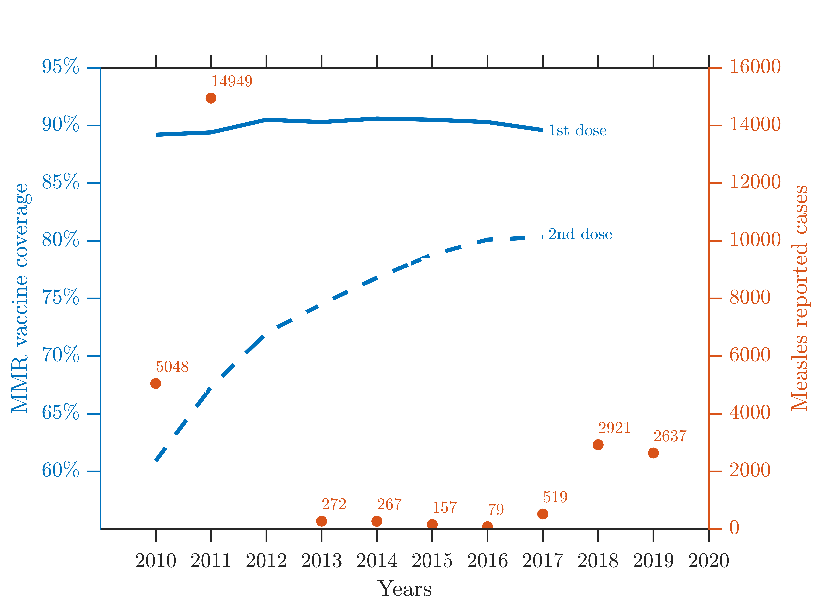
\includegraphics{Figures/Vaccine/Measles_FR}
	\captionsetup{width=0.85\textwidth}
	\caption[MMR vaccine coverage and measles cases in France]{%
		{\bf MMR vaccine coverage and measles cases in France}\\
	In blue, the coverage for the first (solid line) and the second recommended doses (dashed line) of MMR vaccine, among 2-year-old children, for the period 2010--2017~\cite[]{SPF_CouvertureROR2019}. In red, the reported cases of measles in France, for the period 2010--2019~\cite[]{WHO_MeaslesFrance2020}; N.B. no data was reported to the WHO in 2012. The coverage of the first  recommended dose of MMR has been stable, around 89\%, while the coverage of the second dose increases, but remains below 80\%. These low vaccine coverages do not allow epidemic elimination. Indeed, large outbreaks occurred during the period 2010--2011, and again from 2018 on~\cite[]{WHO_MeaslesFrance2020}.}
	\label{fig:Measles_France}
\end{figure}



\section{Objectives}
\label{Vaccine:Objectives}
The objective of the first part of my PhD was to reassess the impact of voluntary vaccination on treatable childhood disease transmission. First, we aimed to build a model combining game theory with an infectious disease transmission model, in order to study the epidemic dynamics as a result of the individual-level decision-making on whether or not to adopt vaccination against childhood infectious diseases. Then, we aimed to determine whether and how could voluntary vaccination avert the epidemic.

In particular, we intended to apply our results to the epidemiology of an infectious disease preventable by vaccination, allowing to discuss the possibility of epidemic elimination. We thus chose to apply our results to the epidemiology of measles.



\section{Published article}
\label{Vaccine:Article}

A scientific article titled ``Prevention of treatable infectious diseases: a game-theoretic approach'' \cite[]{Jijon2017} was published in the journal \textit{Vaccine}. The complete article is available from page~\pageref{articlepdf:1}.

\subsection{Description of the article}
A brief overview of the literature regarding the modeling of infectious diseases and voluntary vaccination is found in the introduction. We propose a model combining game theory with an infectious disease transmission model, in order to study the epidemic dynamics as a result of the individual-level decision-making on whether or not to adopt vaccination against childhood infectious diseases. A flow chart representing the compartmental model for the disease transmission at the population level is depicted in~\figref{fig:Vaccine_FlowDiag}, in the \nameref{Vaccine:Appendix} section of this chapter. 
%  
We present in detail the methods used to compute the voluntary vaccination coverage and to determine the conditions ensuring epidemic elimination. 
An application of the model to the epidemiology of measles is provided. The paper includes a discussion on public policies that may be implemented in high-income settings in order to increase vaccine adoption.

\subsection{Results statement}
\label{Vaccine:Results}

Adding the decision-making model to the classical disease-transmission model provides an estimate of the vaccination coverage that can be reached voluntarly, as a function of the relative cost of vaccination versus treatment, perceived by individuals. Therefore, the relative cost became the parameter to be tuned to increase vaccination coverage.

Our model provides lower bound estimates for the vaccine efficacy and the duration of vaccine-induced immunity, as well an upper bound for the relative cost of vaccine versus treatment, in the context of epidemics controlled by vaccination. These parameters are expressed as functions of the basic reproduction number, i.e., the epidemic severity before the introduction of preventive methods. 

According to our findings, voluntary-vaccination programs can successfully avert epidemics if vaccines are highly efficient, the vaccine-induced immunity is long-lasting and they are delivered at low perceived cost. However, epidemic elimination may only be temporary (cf.~\figref{fig:Vaccine_Bifurcation} in the \nameref{Vaccine:Appendix}) and active efforts from public health authorities are needed to maintain the perceived cost of vaccination low. 

%See~\figref{fig:Vaccine_Bifurcation} in the \nameref{Vaccine:Appendix} section for a depiction

%All results were obtained analytically, providing insight into the mathematical properties of the model. 

\subsubsection*{Application to measles}
We applied our methods to the epidemiology of measles. Our findings suggest that measles elimination was possible thanks to the very long-lasting immunity induced by the MMR vaccine, as well as to the relative cost of vaccination versus treatment which was certainly perceived as low during the mass-vaccination programs of the 90's. 

However, a decrease in vaccine coverage has been observed in several high-income countries. We conclude that reducing the cost of vaccination perceived by individuals in the current context, where measles disease and its sequelae have been less witnessed, may help reaching epidemic elimination through voluntary vaccination, and maintaining elimination status in the long run. For instance, by maintaining the population informed about measles epidemiology in the pre-vaccination era, the disease burden and measles-vaccine high-performance.


%\includepdf[addtotoc = {1,subsection,1,Article,articlepdf:1},
%		addtolist = {%
%			3, figure, The endemic prevalence, fig:Vaccine_1,
%			4, figure, The probability that individuals get effectively vaccinated, fig:Vaccine_2},
%		frame = false,
%		link = true,
%		linkname = Article1,
%		offset = 0cm -0.5cm,
%		height = 26cm,
%		openright = false,
%		pagecommand = {},
%		pages=-]
%		{Parts/Documents/Article1_Vaccination}
%%		{DRAFT_FigsAndDocs/DOC.pdf}

\section{Additional material}
\label{Vaccine:Appendix}
\subsection{Additional figures}

\subsubsection*{Disease transmission flow diagram}
\begin{figure}[H]
	\centering
	%% DRAFT	
%	
\includegraphics[width=0.6\textwidth]{DRAFT_FigsAndDocs/FIG}
	%%
	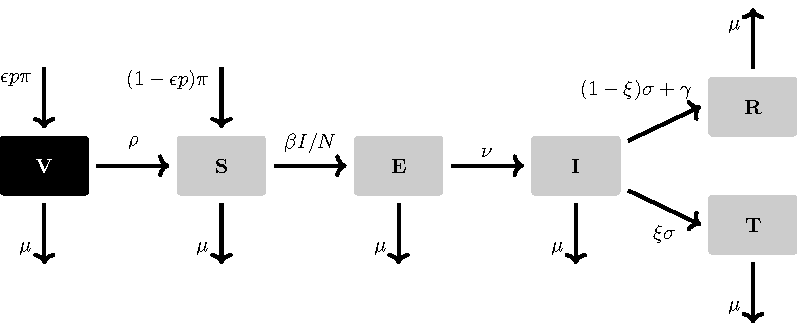
\includegraphics[width=0.8\linewidth]{Figures/Vaccine/Tikz_FlowDiagram/FlowDiagram}
	\caption[Flow diagram for the compartmental model of vaccination against childhood infectious diseases]{%
	       {\bf Flow diagram for the compartmental model of vaccination against childhood infectious diseases}\\
	This flowchart depicts to the ODE system~\hyperlink{Article1.2}{(1)} of the article. Newborns can get vaccinated ($V$) or remain susceptible ($S$). Recently infected individuals ($E$) pass through a latent stage of infection. Then, they become infectious ($I$) and can recover naturally ($R$) or get on treatment ($T$). $N$ denotes the total population. We use $p$ for vaccine coverage, $\epsilon$ for vaccine efficacy and $\rho$ for the rate of vaccine-induced immunity waning. The parameter $\pi$  stands for the inflow of newborns, $\mu$ for the disease-unrelated death rate, $\beta$ for disease transmissibility, $\nu$ for the progression through the latent stage, $\sigma$ is the rate at which individuals start treatment and $\gamma$ is the natural recovery rate. Treatment efficacy is noted~$\xi$.
}
	\label{fig:Vaccine_FlowDiag}
\end{figure}

\newpage
\subsubsection*{Bifurcation diagram}
\hyperlink{fig:Vaccine_Bifurcation}{Fig.~\ref*{fig:Vaccine_Bifurcation}} is a variation of~\hyperlink{fig:Vaccine_1}{fig. 1 of the article} which allows to visualize the stability of the ODE system equilibria and the loss of stability of the DFS when the decision model is coupled to the transmission model.

\begin{figure}[H]
	\centering	
	%% DRAFT
%	
\includegraphics[width=0.4\textwidth]{DRAFT_FigsAndDocs/FIG}
	%%
	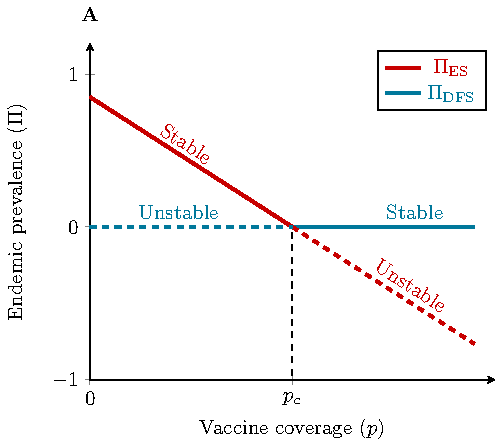
\includegraphics[width=0.4\linewidth]{Figures/Vaccine/TikZ_Bifurcation/TranscriticalBifurcation}
	\hspace{1cm}\
	%% DRAFT
%	
\includegraphics[width=0.4\textwidth]{DRAFT_FigsAndDocs/FIG}
	%%
	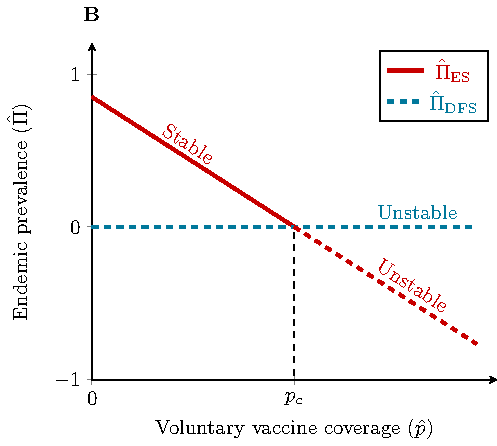
\includegraphics[width=0.4\linewidth]{Figures/Vaccine/TikZ_Bifurcation/TranscriticalBifurcation_WithGame}
	\caption[ Bifurcation diagram for the endemic prevalence]{%
		{\bf Bifurcation diagram for the endemic prevalence}\\
	The disease-free state (DFS) and the endemic state (ES) are depicted in blue and red, respectively. A change in the stability of the system's equilibria occurs when the vaccine coverage reaches the critical value $p_c$ (i.e., when the effective reproduction number equals to 1), which is depicted by the transition from a solid to a dashed line. \textbf{(A)} The bifurcation diagram for the endemic prevalence, for the model without the individual-level decision-making component. \textbf{(B)} The bifurcation diagram for the endemic prevalence induced by voluntary prevention, $\hat{\Pi} \equiv \Pi(\hat{p})$. The stability of the DFS for $\hat{p} \geq p_c$ is lost when the game is coupled to the compartimental model: there exists no equilibrium coverage for voluntary vaccination once the epidemic has been averted.}
	\label{fig:Vaccine_Bifurcation}
\end{figure}

\section{Further discussion}

%\subsection{The French mistrust in vaccination}
%The reasons of included doubts on the immunization programs recommended by health authorities and.

\subsection{A note on mandatory vaccination}

Here, we discuss briefly the results of implementing mandatory vaccination, as an alternative to allowing individuals to decide whether or not to adopt recommended immunization programs.

Some countries have witnessed infectious diseases reemergence and have established mandatory vaccination as a result. As of 2018, vaccination against measles was mandatory in 9 European countries. In 2019, France had added 8 mandatory vaccines to a list of 3, and Italy had established 10 mandatory vaccines~\cite[]{Bechini2019}. The most common strategies to enforce vaccination have been implementing monetary fines to parents who do not vaccinate their children, excluding unvaccinated children from school~\cite[]{Drew2019,Bechini2019} and withholding public financial child support~\cite[]{Drew2019,Australia2015}.

Italy, France and Australia have witnessed an increase in MMR vaccine coverage following mandate establishment. However, it is not clear whether this coverage level will last in the future. In addition, mandatory vaccination may not always accomplish the objective of increasing vaccination coverage. For instance, in California, in the US, the number of unvaccinated children that were home-schooled quadrupled between September 2016 and August 2019~\cite[]{Drew2019}. 

Hence, mandatory vaccination may not solve the issues that lead to non-vaccination and may increase health disparities between individuals. Experts thus believe that mandatory vaccination should be a temporary mesure only~\cite[]{Bechini2019}. Instead of mandates enforcing vaccination, increasing vaccination coverage through the voluntary participation of individuals would require allocating ressources towards facilitating access to vaccination and information campaigns to address vaccine hesitancy~\cite[]{Drew2019,Bechini2019}. These arguments highlight the importance of addressing the individuals' decision-making on vaccination adoption and the pertinence of our results.